%!TEX root = ../booklet.tex
% ^ leave for LaTeXTools build functionality

\definecolor{darkGreen}{RGB}{20,100,1}

\begin{puzzle}
  A standard six-sided die has a \textbf{planar unfolding} of this form,
  created by cutting along some of the edges and flattening the faces into
  a plane:

  \vfill

  \centerImg{2in}{aDiceySituation/diceExample.pdf}

  \vfill

  In the following images, three different-colored standard dice have been
  moved on an $8\times 8$ board:
    \textcolor{red}{red},
    \textcolor{darkGreen}{green}, and
    \textcolor{blue}{blue}.
  Two of the dice in each figure are moved by ``rolling'' the dice carefully
  from square to square as in the following image.

  \vfill

  \centerImg{4in}{aDiceySituation/diceLegal.pdf}

  \vfill

  However, the third color die in each image was simply picked up
  and placed at its new location. A clue to the location of an
  EXTRA Puzzle may
  be obtained by concatenating the strings of letters associated with this
  third die from each figure. (Look out: the images don't appear in the
  same order as the resulting message.)

  Relay the decrypted message to Game HQ for \(100\) points!

  \vfill

  \newpage



  \begin{center}
    \begin{tabular}{c}
      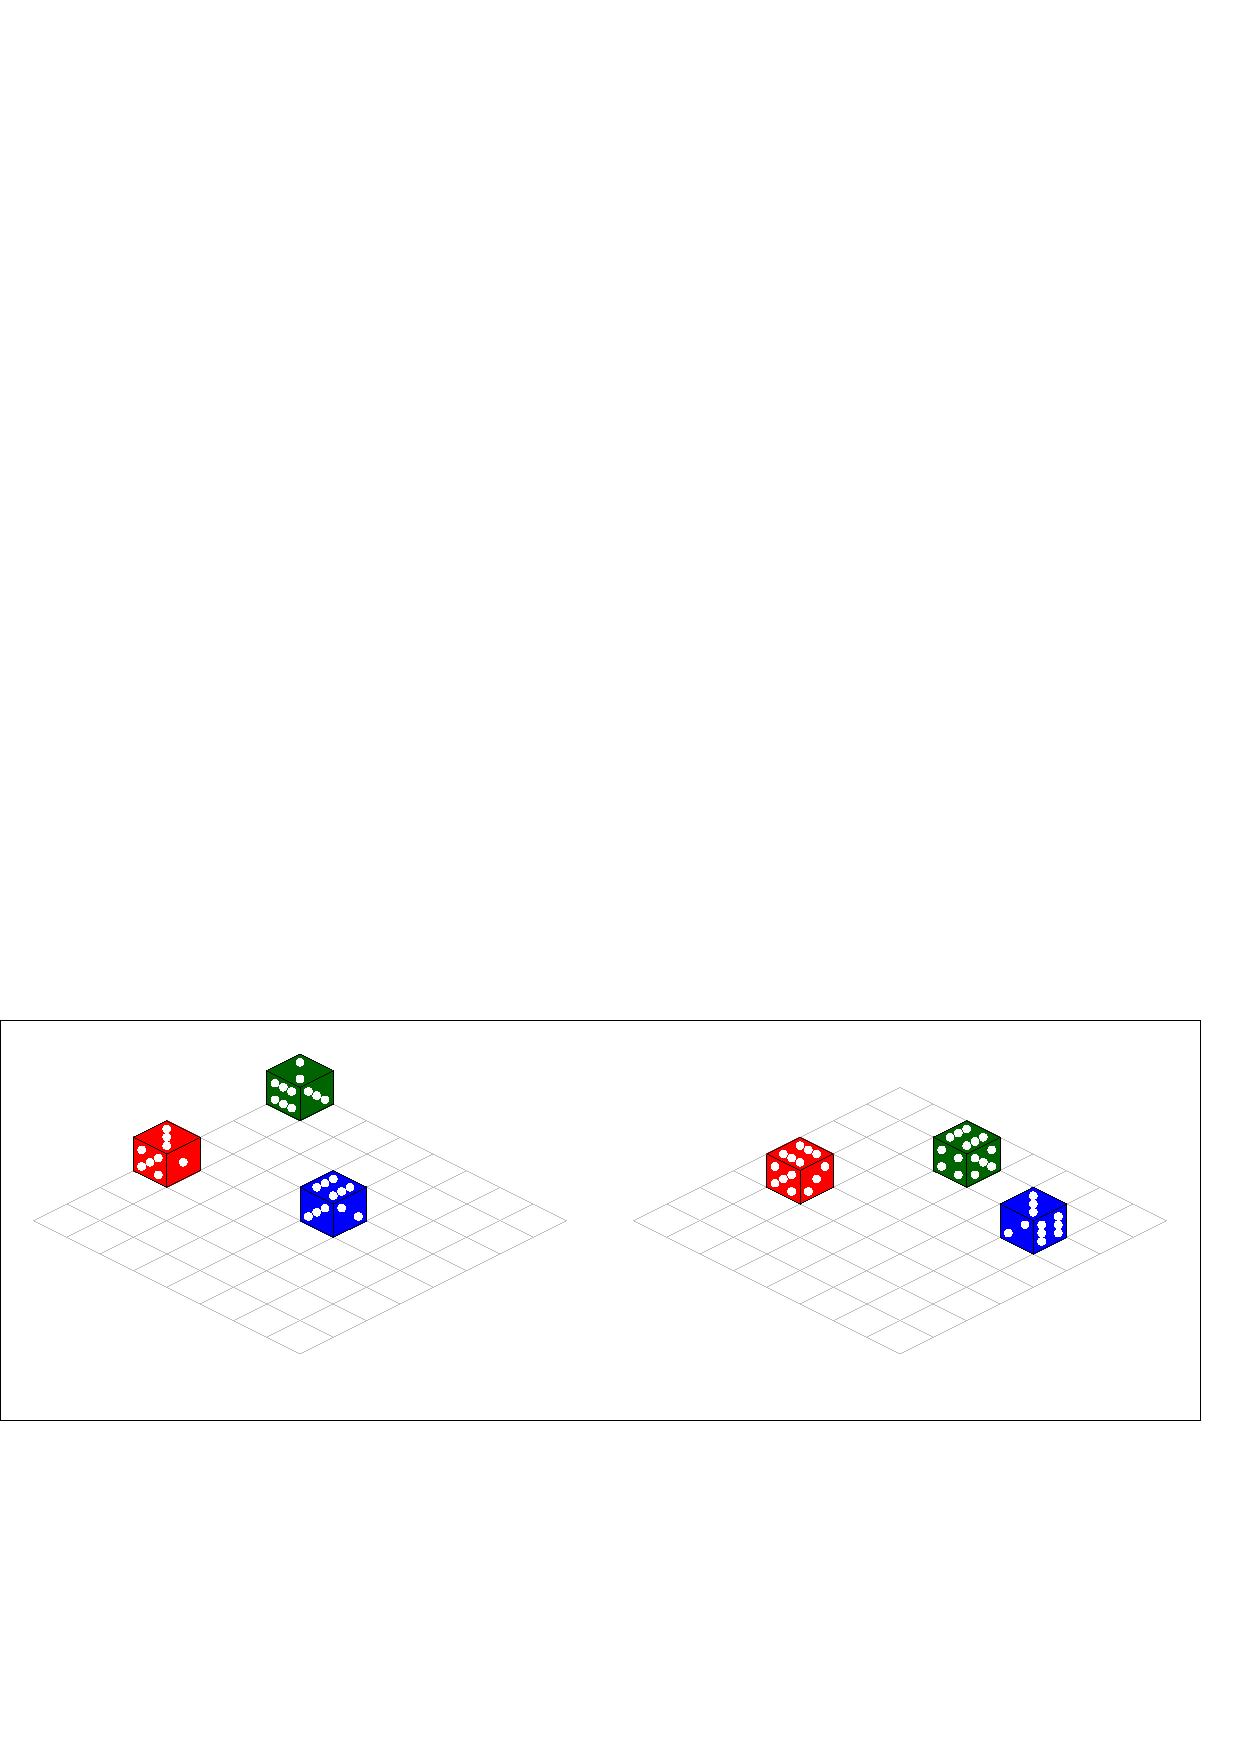
\includegraphics[width=0.8\linewidth]{aDiceySituation/diceBlue02.pdf}
      \\
      \textcolor{red}{JUS} |
      \textcolor{darkGreen}{AST} |
      \textcolor{blue}{GIS}
    \end{tabular}
  \end{center}


  \vfill


  \begin{center}
    \begin{tabular}{c}
      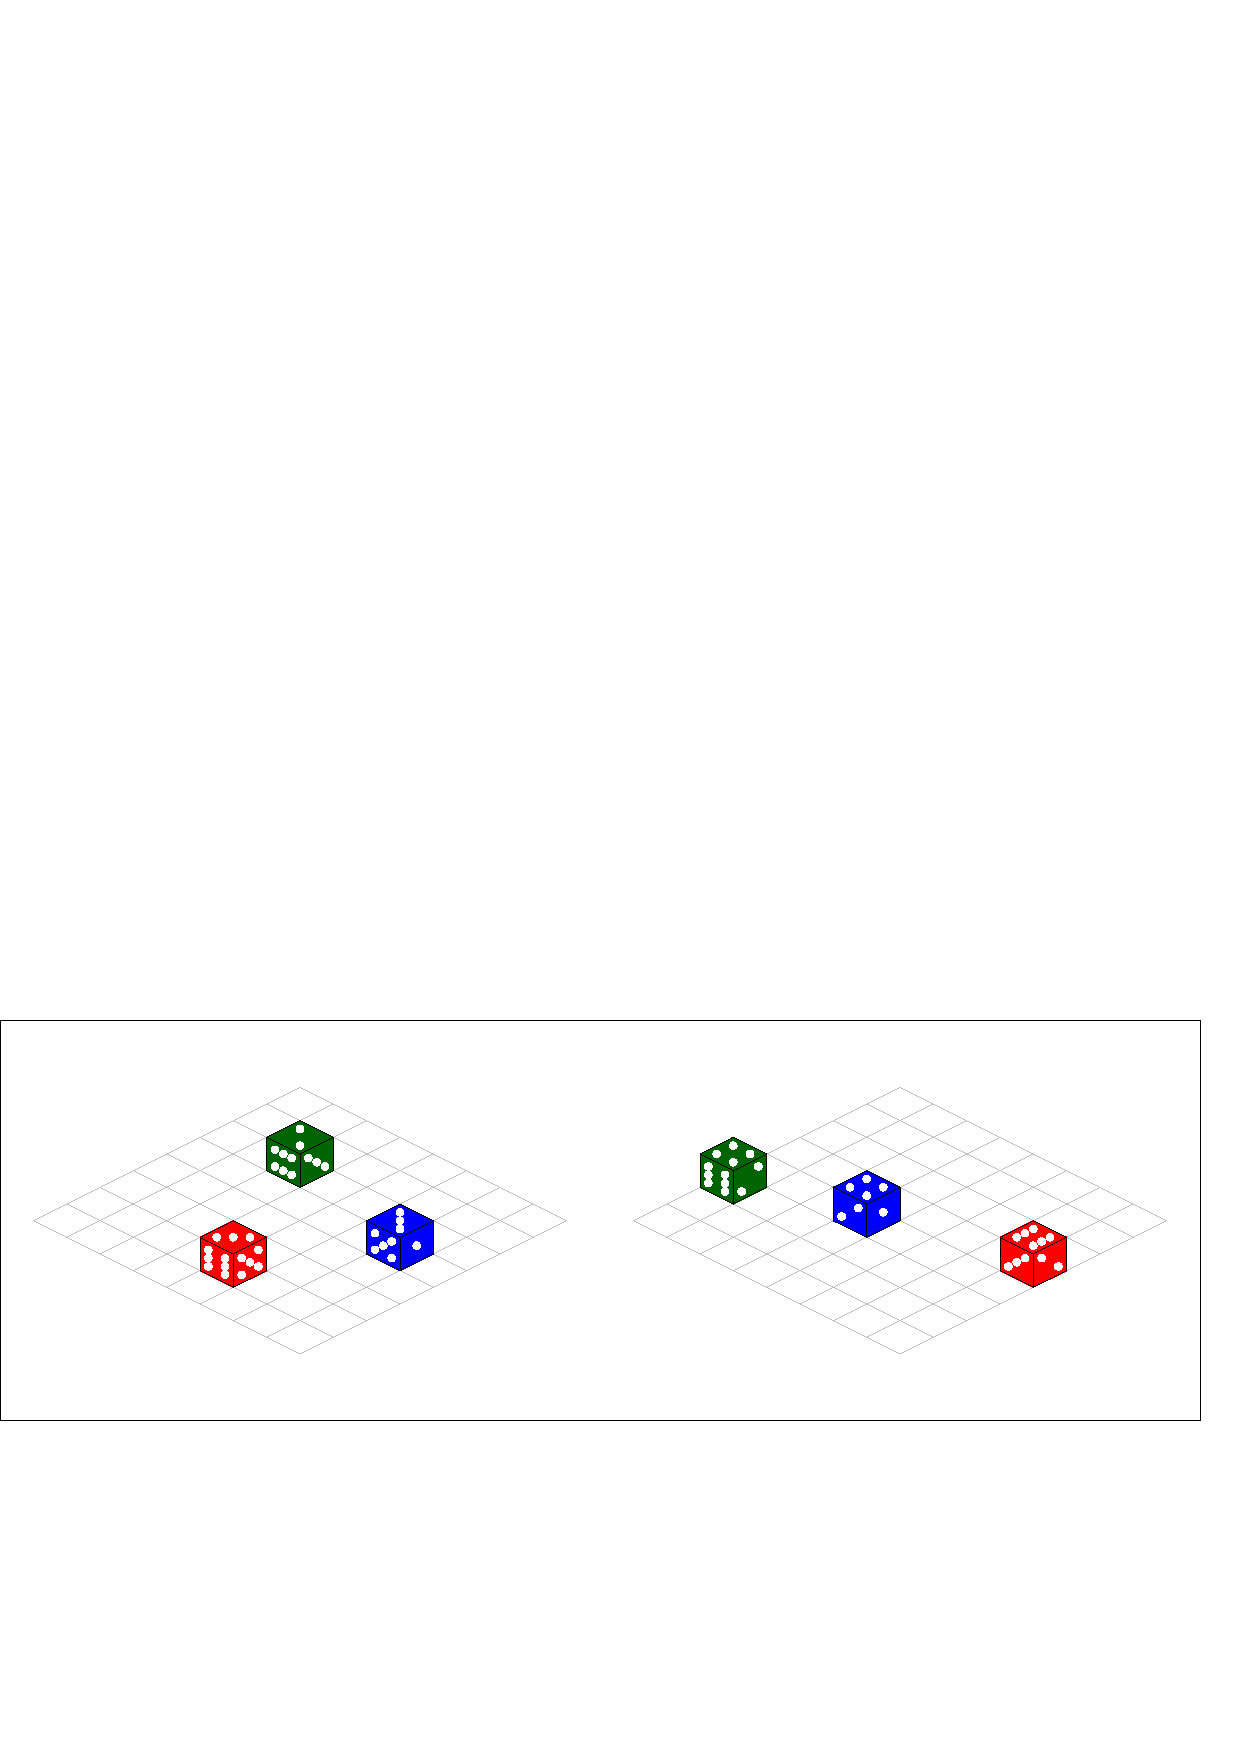
\includegraphics[width=0.8\linewidth]{aDiceySituation/diceRed03.pdf}
      \\
      \textcolor{red}{NOTJ} |
      \textcolor{darkGreen}{TARE} |
      \textcolor{blue}{EDYO}
    \end{tabular}
  \end{center}


  \vfill


  \begin{center}
    \begin{tabular}{c}
      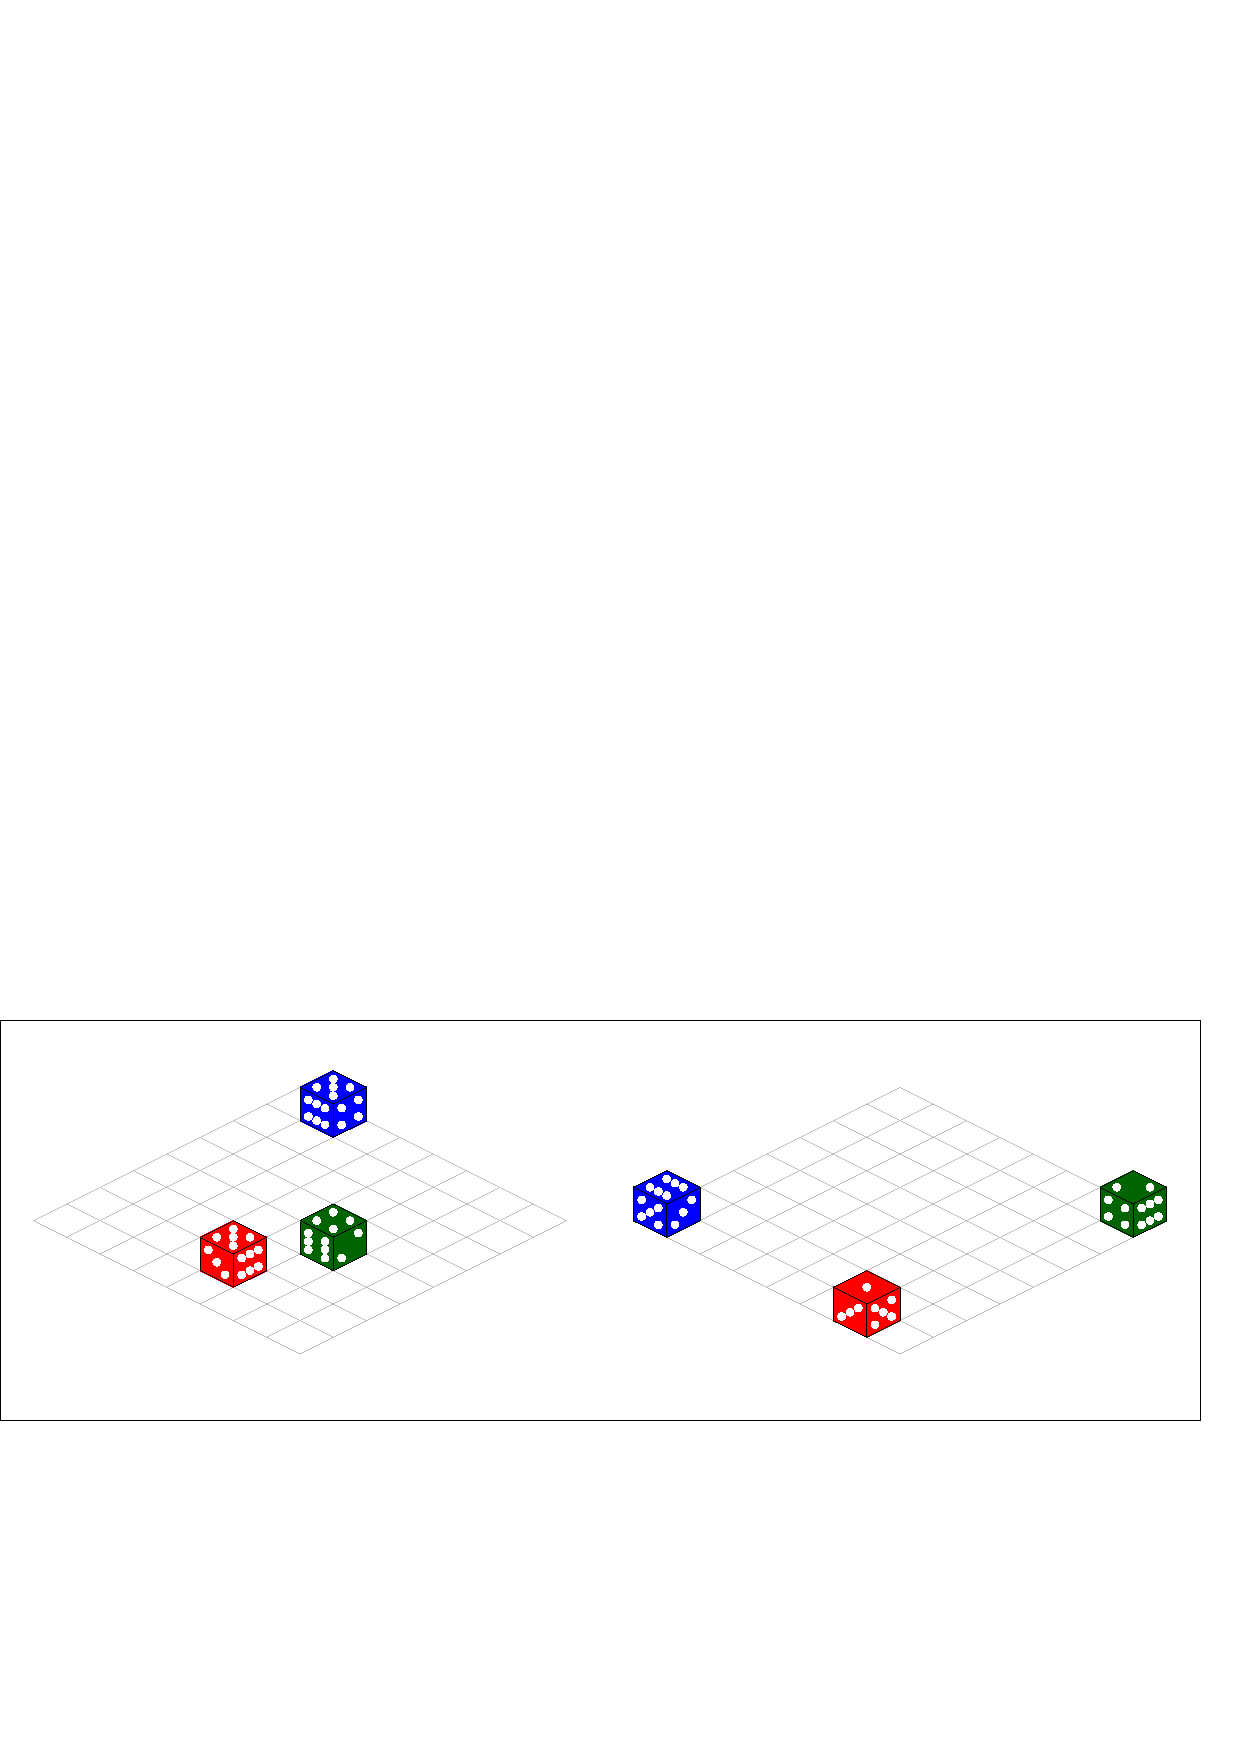
\includegraphics[width=0.8\linewidth]{aDiceySituation/diceBlue03.pdf}
      \\
      \textcolor{red}{DHER} |
      \textcolor{darkGreen}{URTI} |
      \textcolor{blue}{USTB}
    \end{tabular}
  \end{center}


  \newpage


  \begin{center}
    \begin{tabular}{c}
      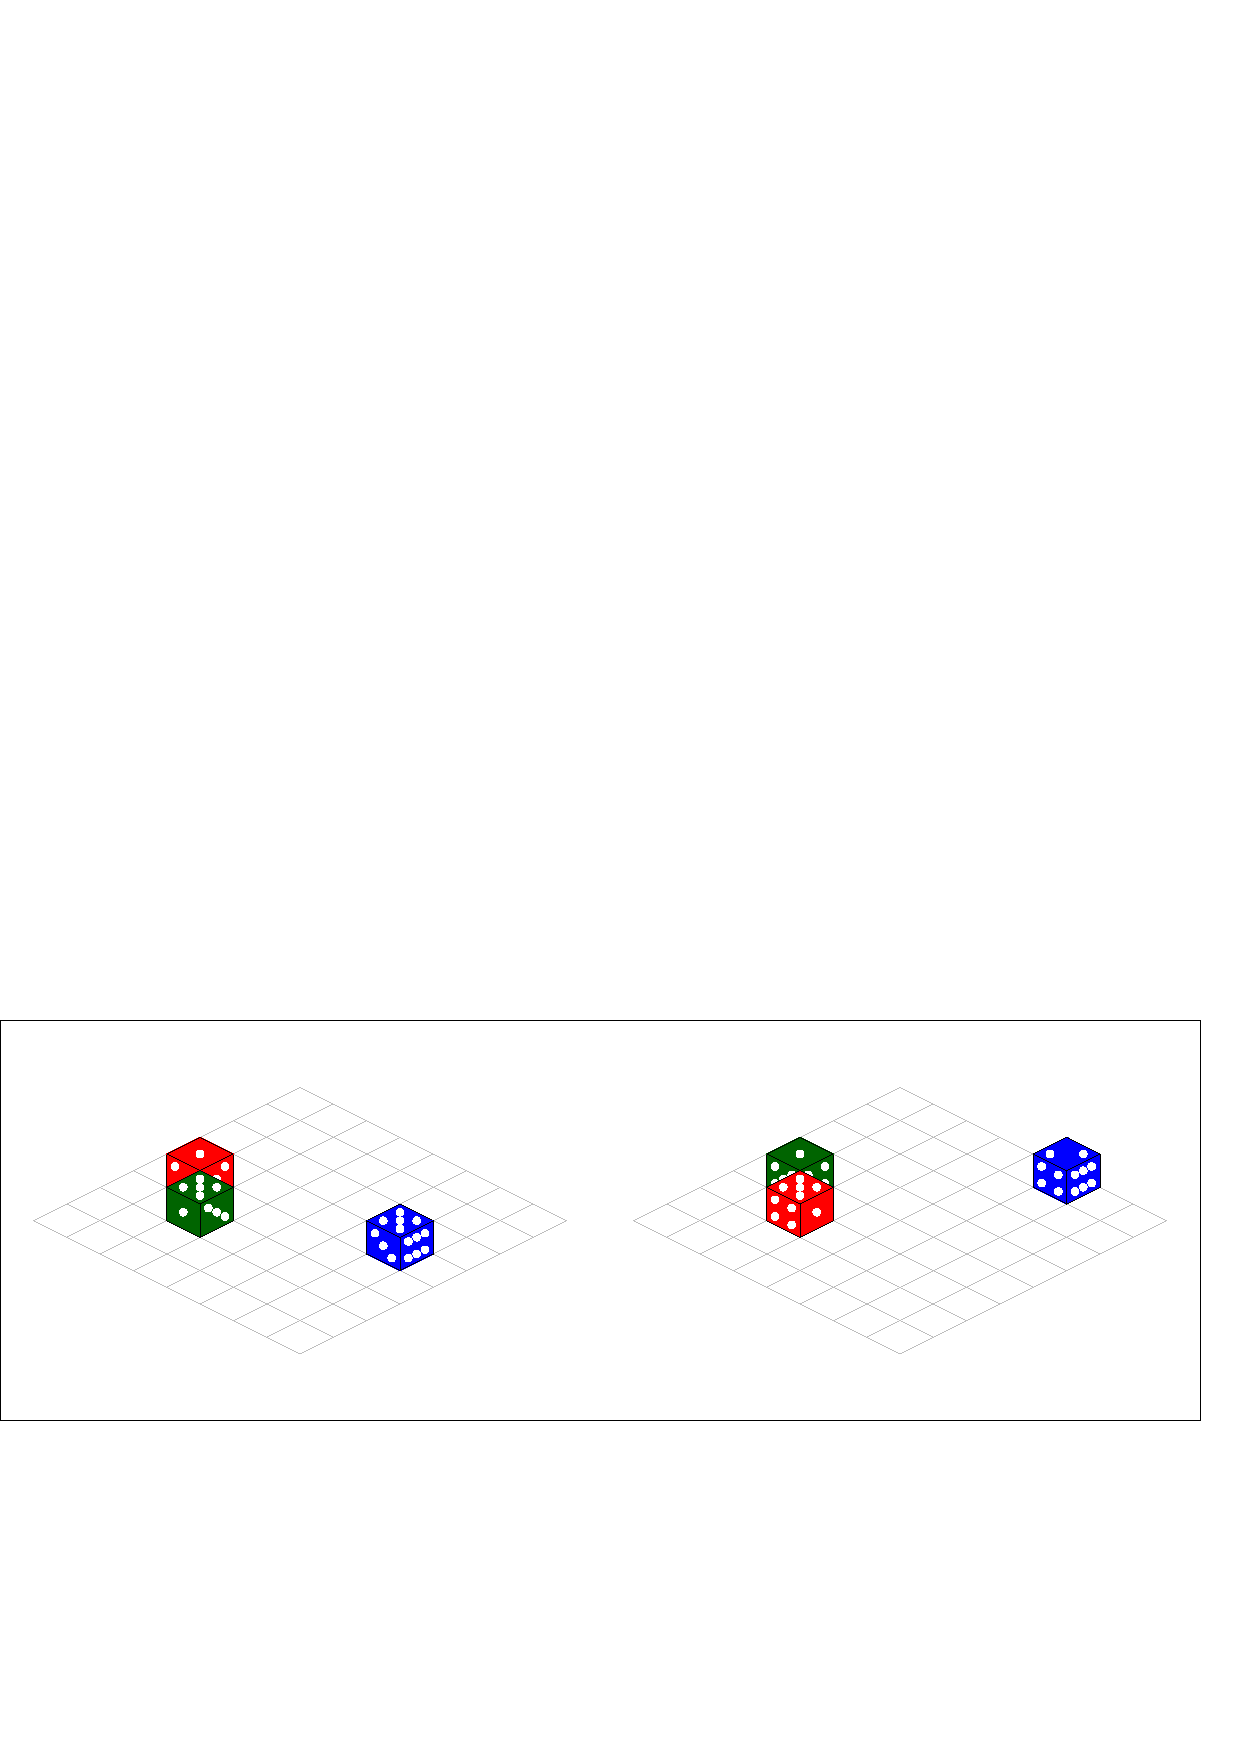
\includegraphics[width=0.8\linewidth]{aDiceySituation/diceGreen02.pdf}
      \\
      \textcolor{red}{MEO} |
      \textcolor{darkGreen}{LAC} |
      \textcolor{blue}{MEO}
    \end{tabular}
  \end{center}


  \vfill


  \begin{center}
    \begin{tabular}{c}
      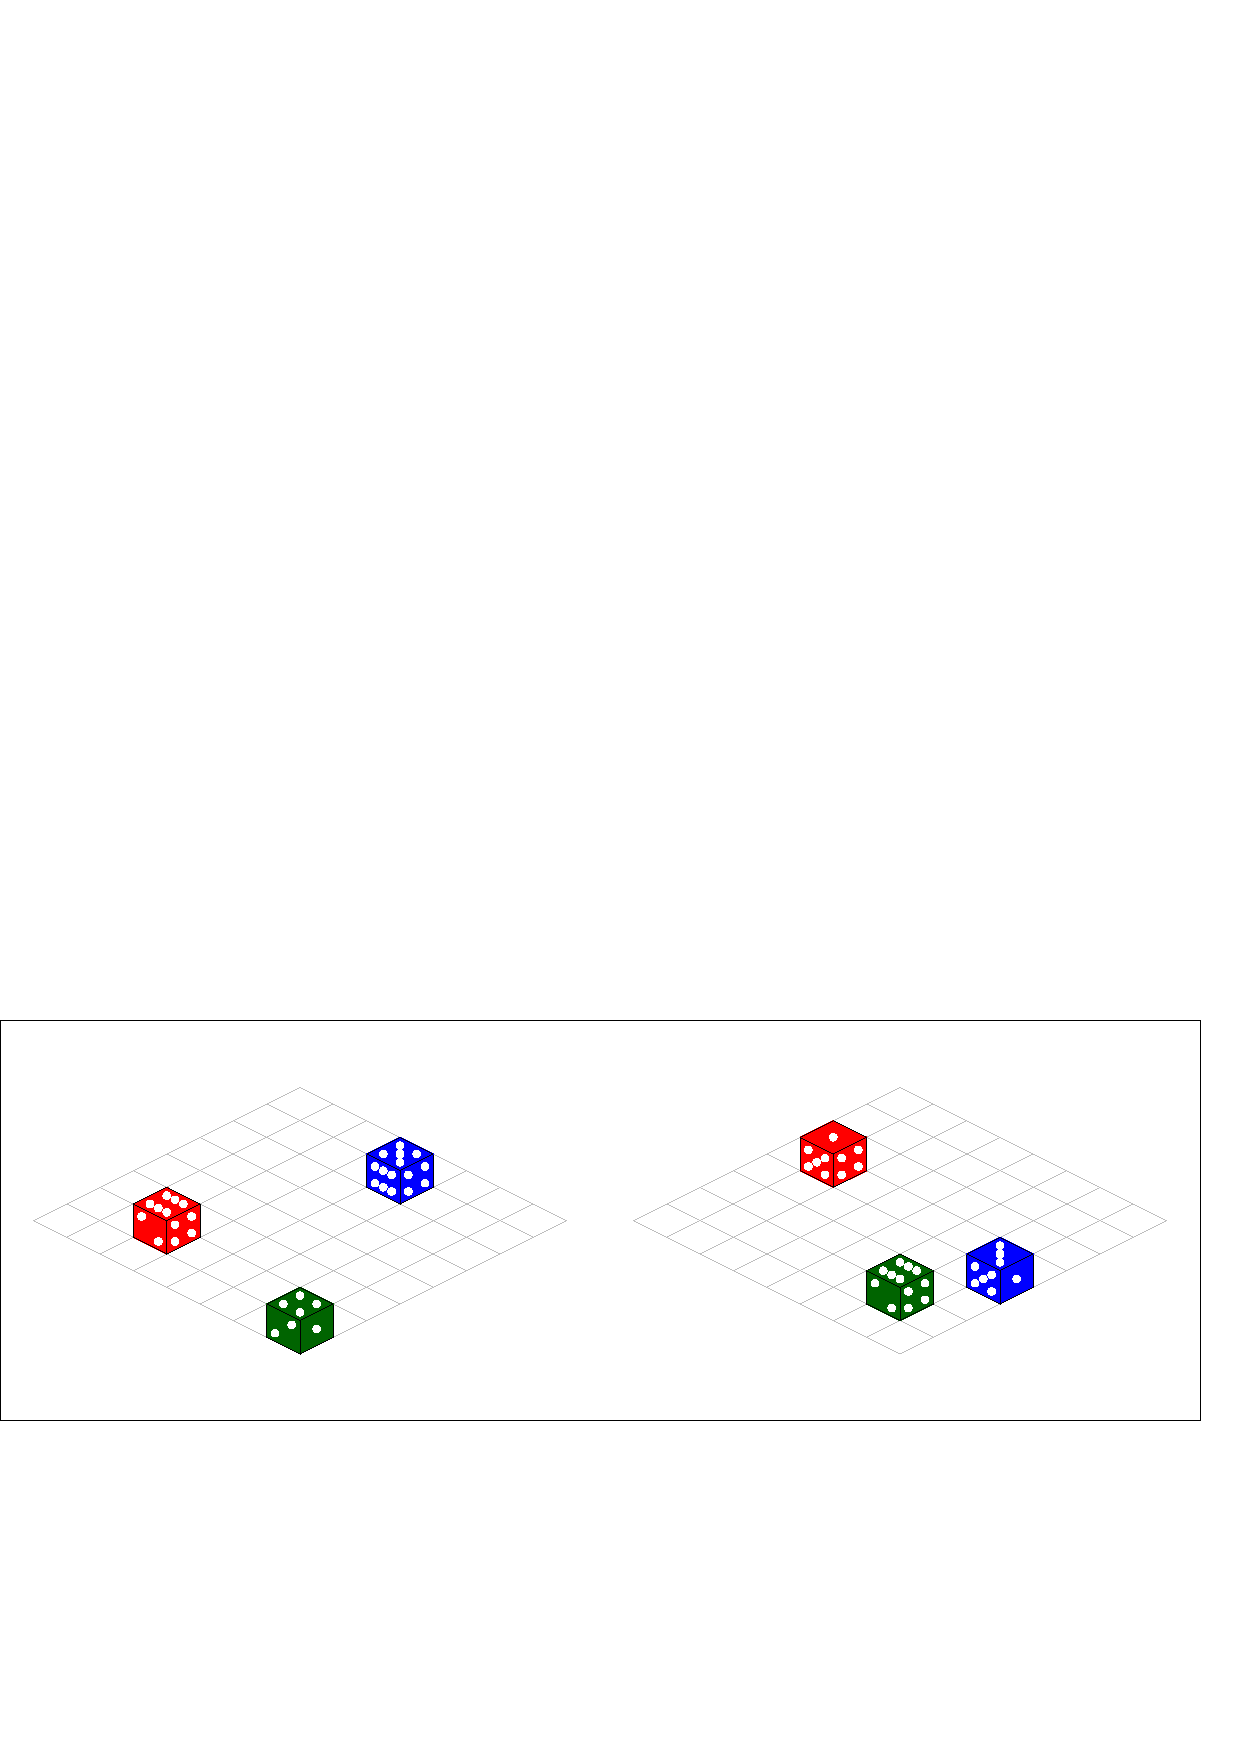
\includegraphics[width=0.8\linewidth]{aDiceySituation/diceGreen01.pdf}
      \\
      \textcolor{red}{YOU} |
      \textcolor{darkGreen}{REA} |
      \textcolor{blue}{YOU}
    \end{tabular}
  \end{center}


  \vfill


  \begin{center}
    \begin{tabular}{c}
      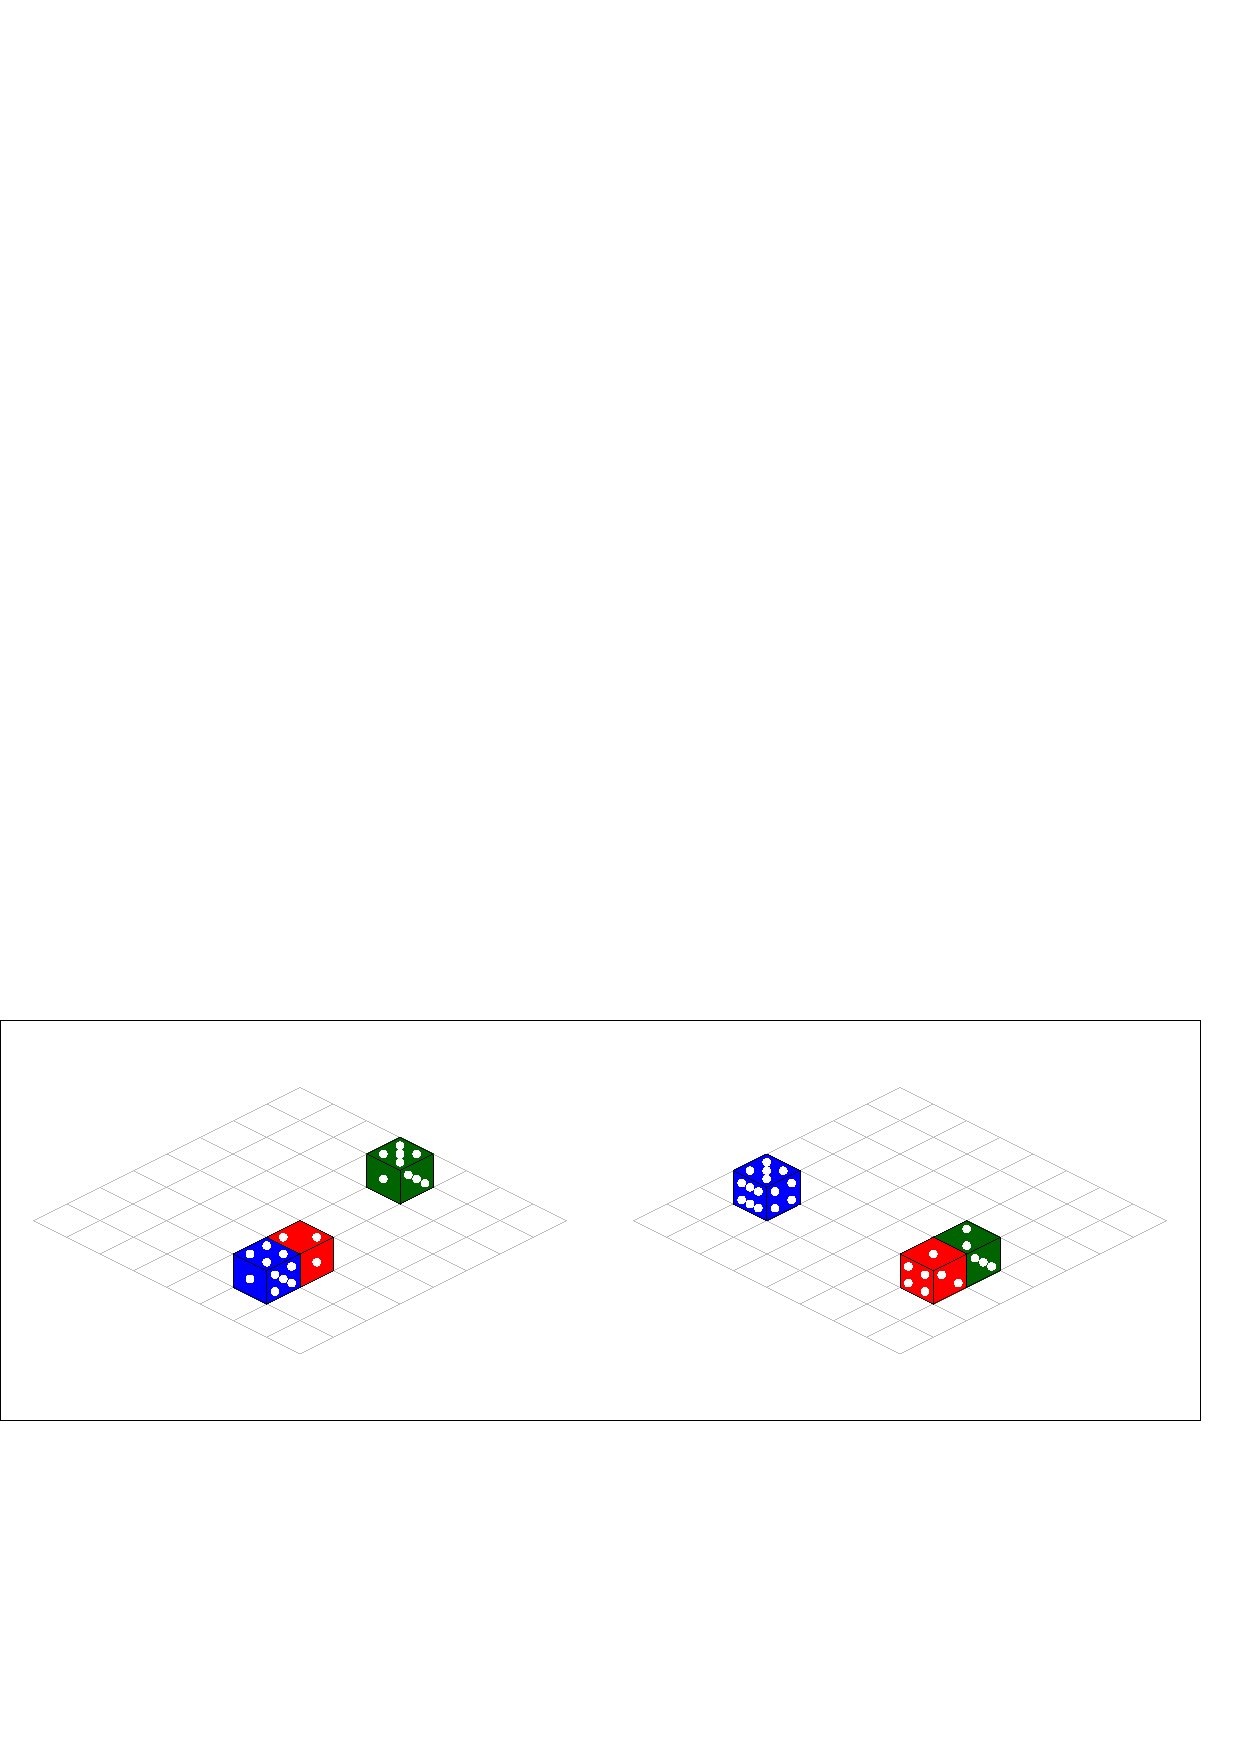
\includegraphics[width=0.8\linewidth]{aDiceySituation/diceGreen03.pdf}
      \\
      \textcolor{red}{ATH} |
      \textcolor{darkGreen}{ITE} |
      \textcolor{blue}{ATH}
    \end{tabular}
  \end{center}


  \newpage


  \begin{center}
    \begin{tabular}{c}
      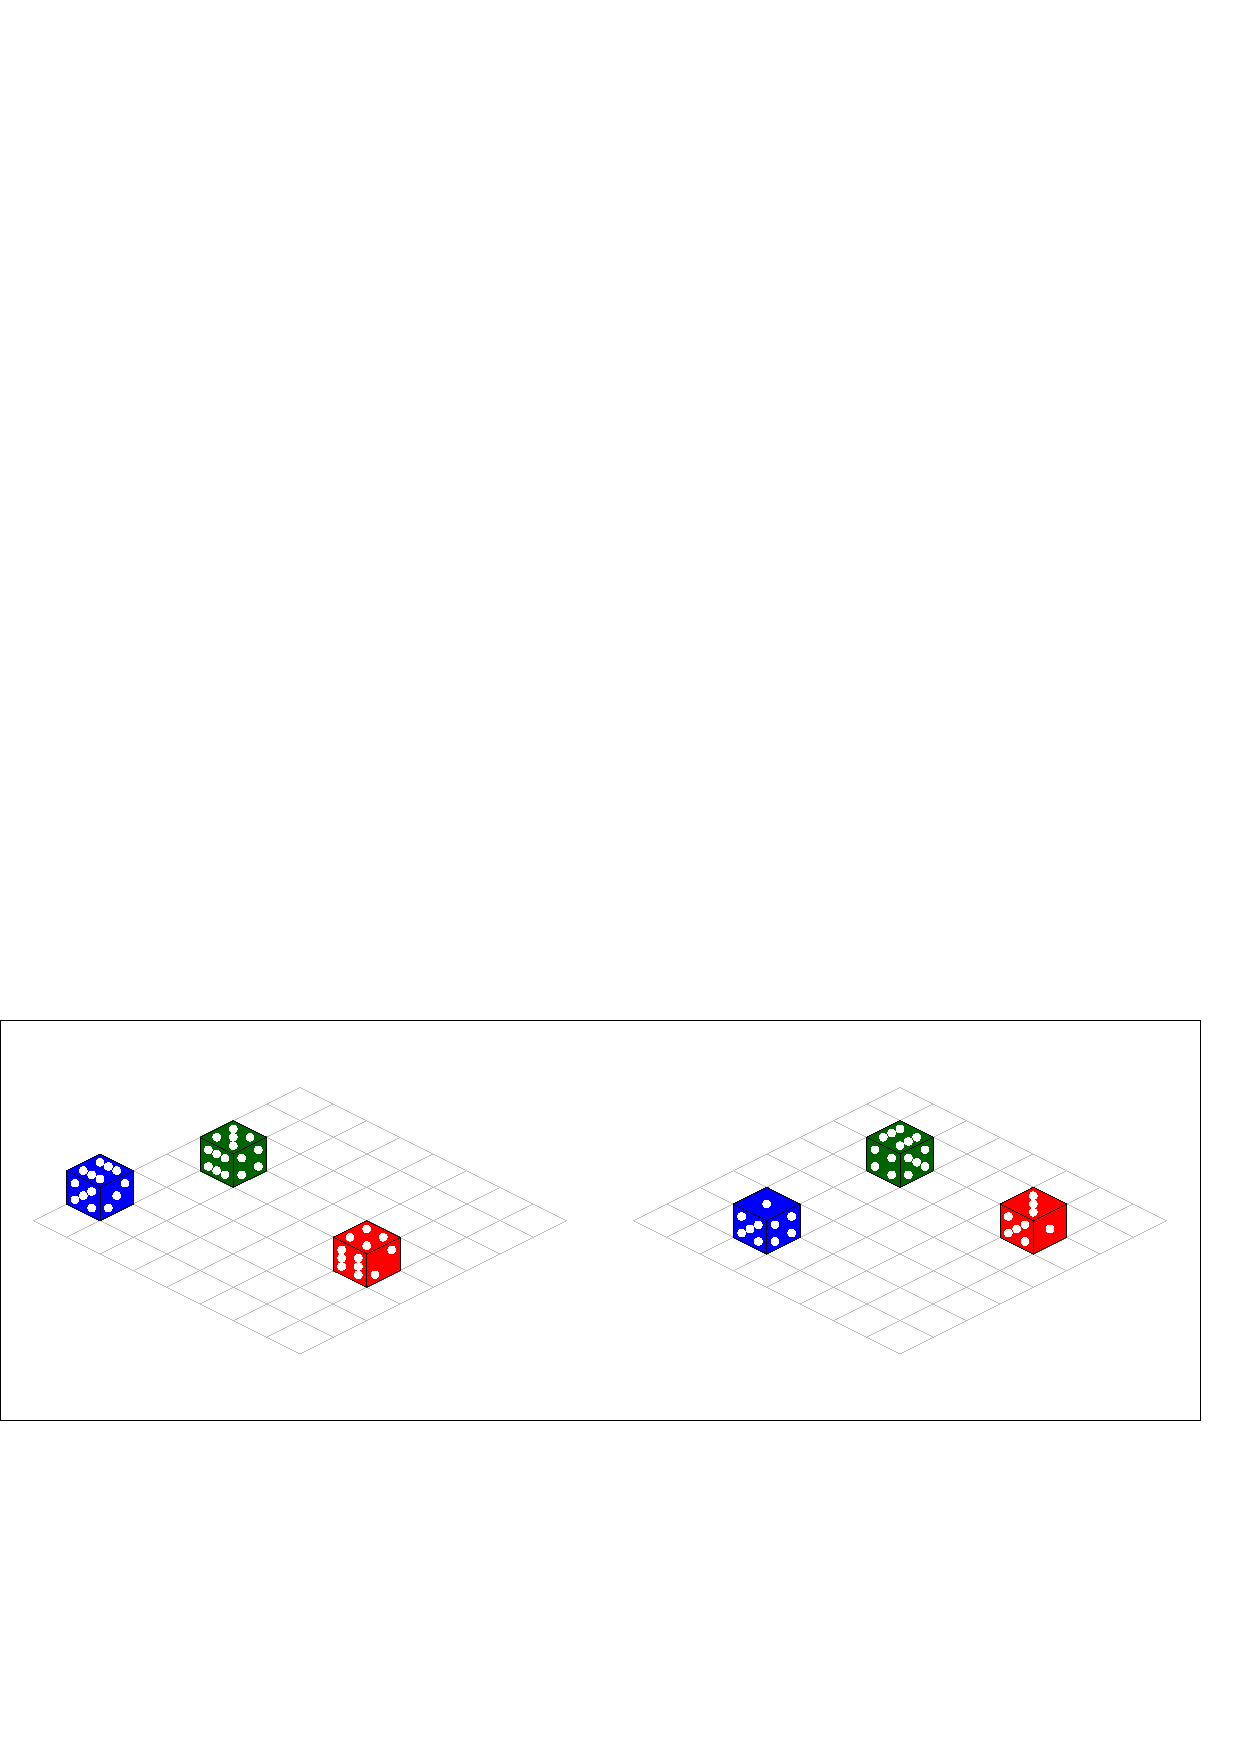
\includegraphics[width=0.8\linewidth]{aDiceySituation/diceRed02.pdf}
      \\
      \textcolor{red}{DIN} |
      \textcolor{darkGreen}{SIS} |
      \textcolor{blue}{VEW}
    \end{tabular}
  \end{center}


  \vfill


  \begin{center}
    \begin{tabular}{c}
      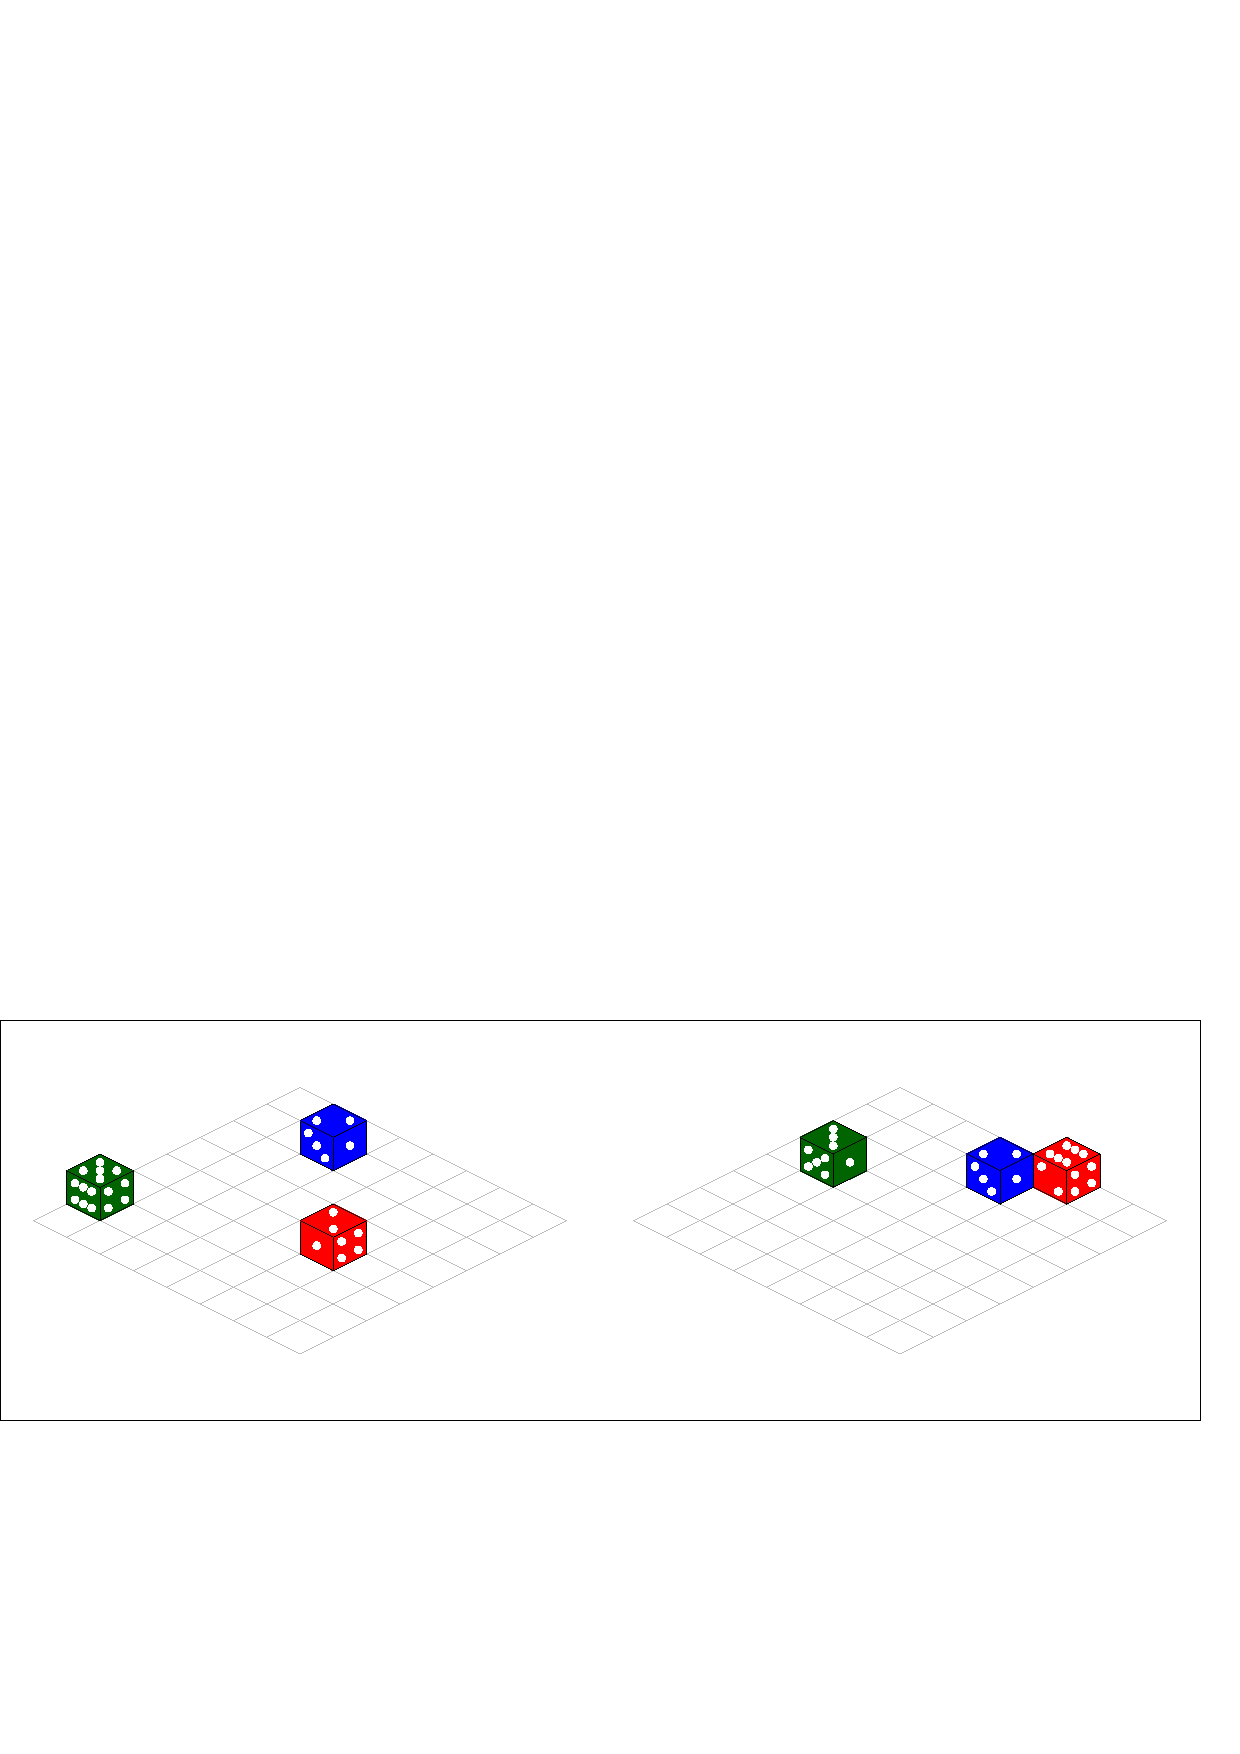
\includegraphics[width=0.8\linewidth]{aDiceySituation/diceRed01.pdf}
      \\
      \textcolor{red}{DWH} |
      \textcolor{darkGreen}{AFR} |
      \textcolor{blue}{ISP}
    \end{tabular}
  \end{center}


  \vfill


  \begin{center}
    \begin{tabular}{c}
      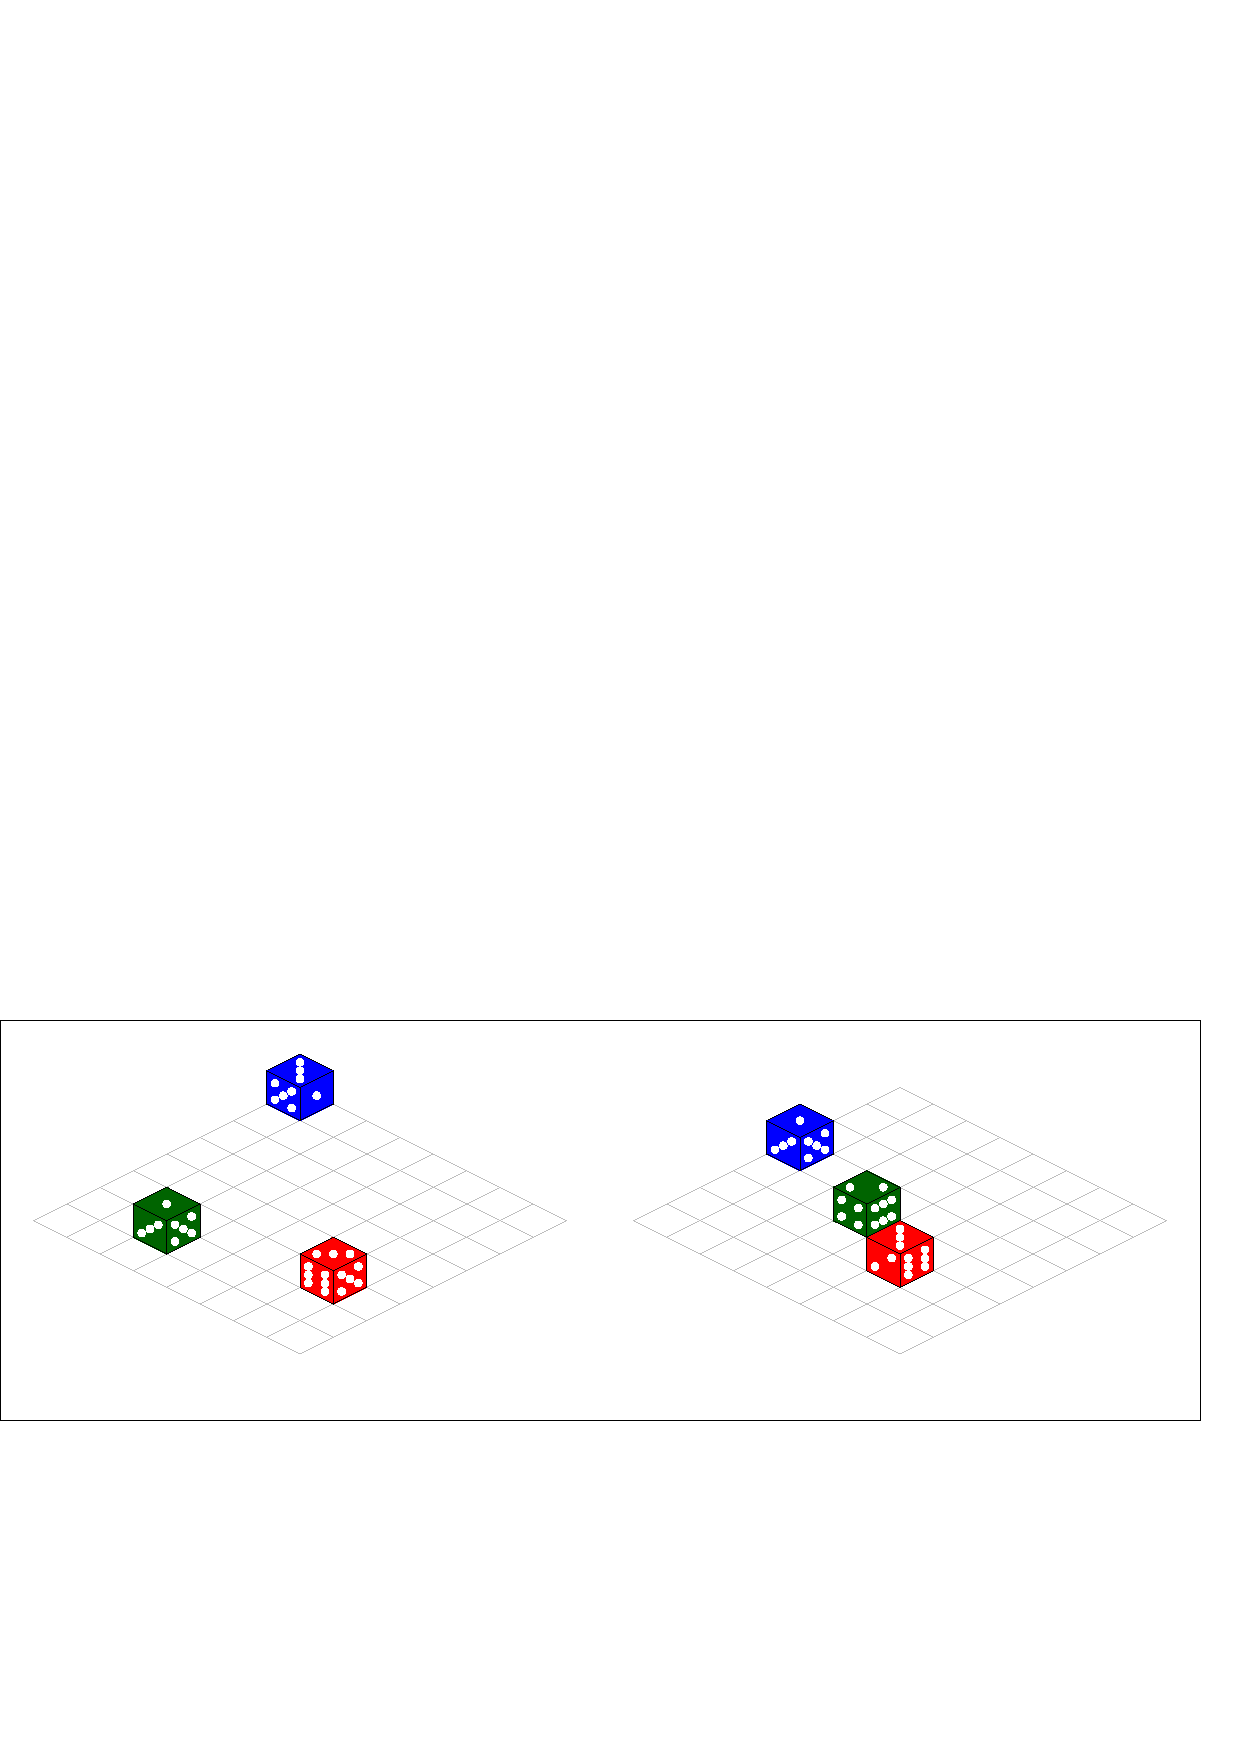
\includegraphics[width=0.8\linewidth]{aDiceySituation/diceBlue01.pdf}
      \\
      \textcolor{red}{GIM} |
      \textcolor{darkGreen}{NTH} |
      \textcolor{blue}{KAN}
    \end{tabular}
  \end{center}

\end{puzzle}

\begin{extraPuzzle}
  Awesome! Did you figure out how to roll two of the dice in every picture,
  or did you find a way to identify which dice movements were impossible?

  Suppose one of those dice was positioned on the \(8\times 8\) grid
  as below. How many different positions and orientations can the die
  be legally moved into by rolling (as in the main puzzle)?
  Report your best guess to Game HQ, and the team(s)
  closest to the correct answer will earn \(50\) bonus points!

  \begin{center}
  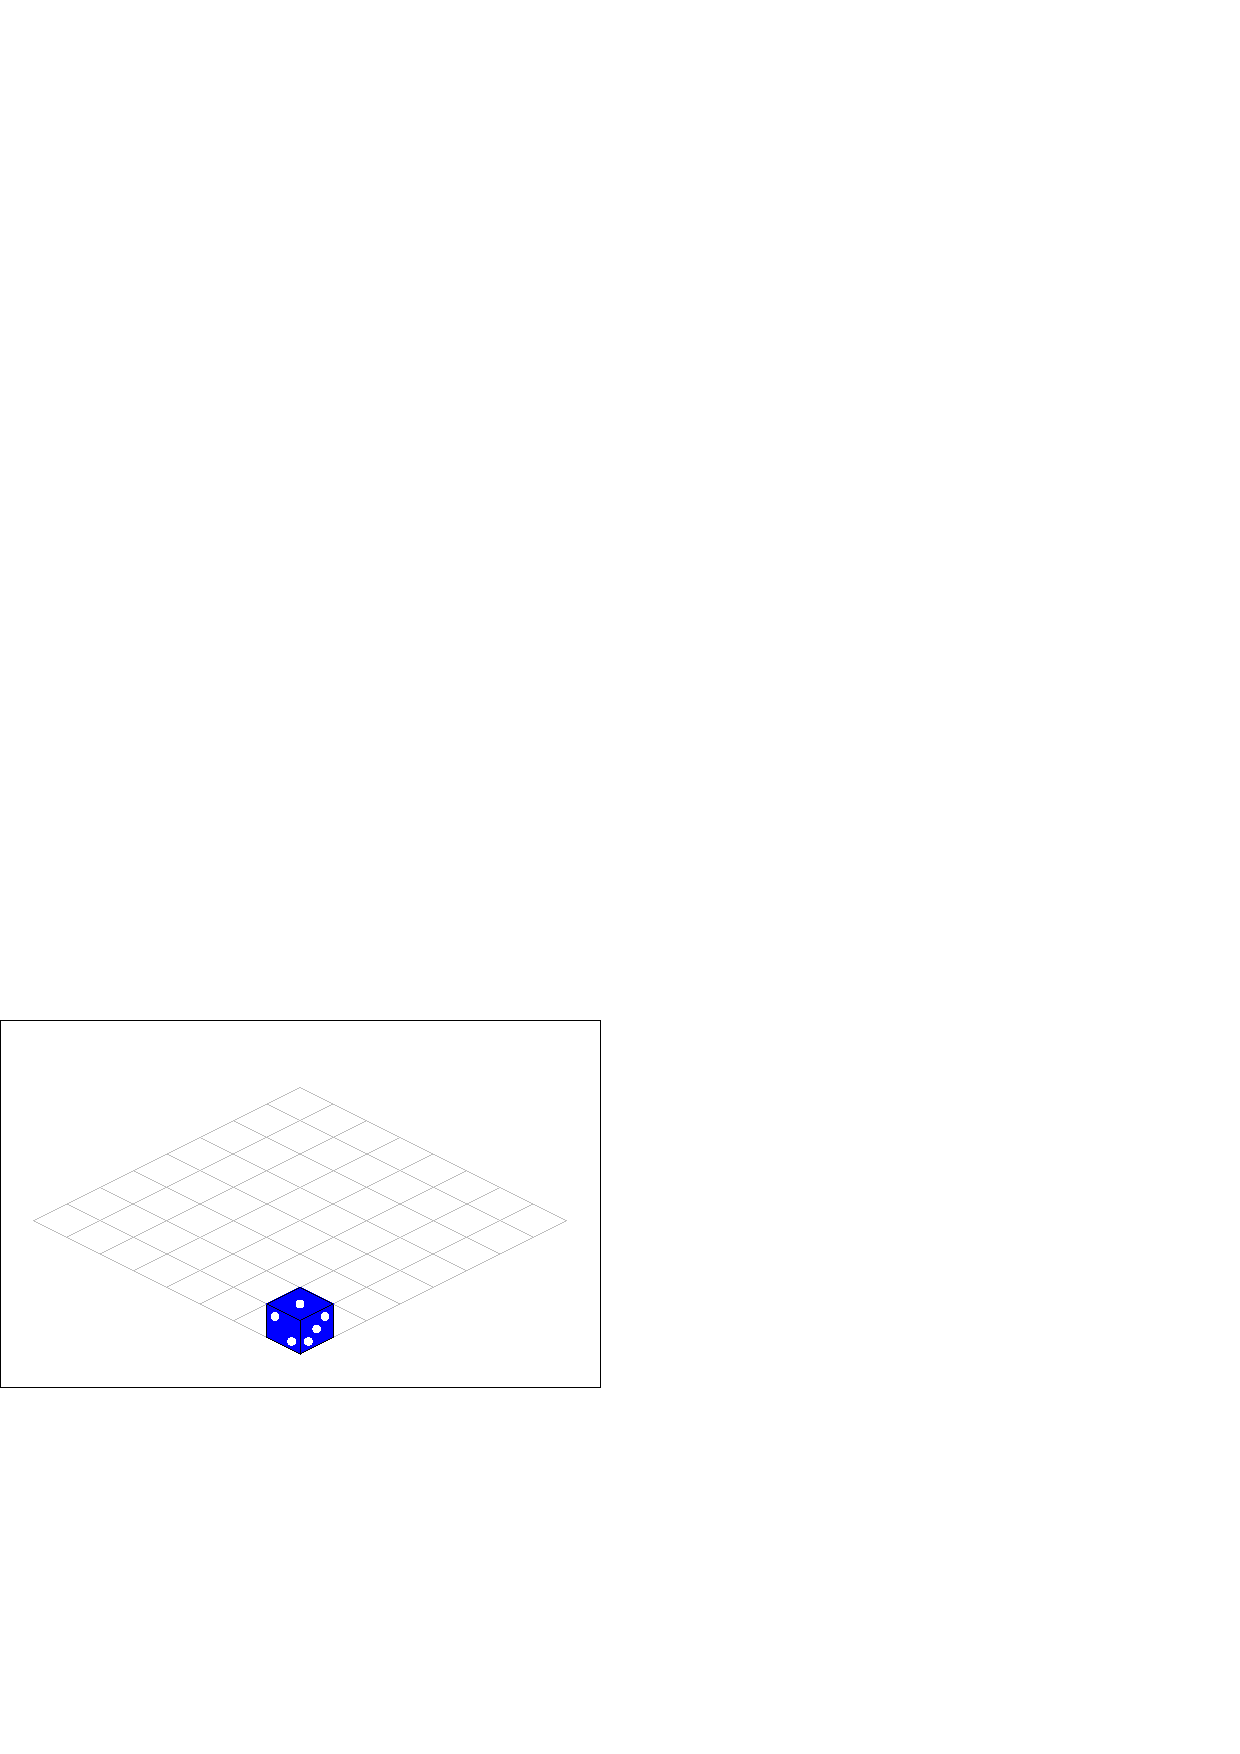
\includegraphics[width=0.8\linewidth]{aDiceySituation/diceExtra.pdf}
  \end{center}
\end{extraPuzzle}